% !TeX root = ../main.tex
% Add the above to each chapter to make compiling the PDF easier in some editors.

\chapter{Related work}\label{chapter:relatedwork}

\section{Background}
In this chapter we will talk about optimization, in particular the field
of linear programming, we focus on
the  most widely used algorithms to tackle this problem,
and we present some use cases and benchmarks for this technique.

\subsection{Linear Programming}
Informally, \gls{lp} is a method to calculate the best possible outcome from a given set
of requirements. A concrete real-world application of such a method is
for instance aiming to maxmize profit in a business, given some constraints on your variables
like raw material availability, labor hours, etc.

Formally, \gls{lp} is a mathematical modeling technique in which
a linear function (called the objective function) \( z: \mathbb{R}^n \to \mathbb{R} \)
is maximized or minimized when subject to a set of linear constraints or inequalities. 
A maximization \gls{lp} problem is then defined as:
Maximize:
\begin{align}
    \text{Maximize} \quad & z = \mathbf{c}^T \mathbf{x} \notag \\
    \text{subject to} \quad & \mathbf{A} \mathbf{x} \leq \mathbf{b} \notag \\
    & \mathbf{x} \geq \mathbf{0} \label{LP_Problem}
\end{align}
Where $n$ is the number of decision variables and $m$ is the number of constraints:
\(\mathbf{x} \in \mathbb{R}^n\) is the column vector of decision variables.
\(\mathbf{c} \in \mathbb{R}^n\) is the column vector of coefficients in the objective function.
\(\mathbf{A} \in \mathbb{R}^{m \times n}\) is the coefficient matrix in the constraints.
\(\mathbf{b} \in \mathbb{R}^m\) is the column vector of the right-hand sides of the constraints.
In the following sections, we focus on \gls{lp} problems that are maximization problems and we primarily
use the matrix representation of the problem.
To derive the setting for our contribution,
we also explore a special instance of \gls{lp} problems called packing \gls{lp}.
\subsubsection{Packing LP}
One LP problem class that we are dealing with is called the packing LP problem. It is a special instance where:
\( \mathbf{c}  = \mathbf{b} =  \begin{bmatrix}
    1 & 1 & \dots & 1
\end{bmatrix} \).
Our specific problem is then expressed as follows:
\begin{align}
    \text{Maximize} \quad   & \sum_{j=1}^{n} x_j \notag                                                     \\
    \text{subject to} \quad & \notag                                                                        \\
                            & \sum_{j=1}^{n} a_{ij} x_j \leq 1, \quad & i = 1, \ldots, m \notag             \\
                            & x_j \geq 0, \quad                       & j = 1, \ldots, n \label{PLP_Problem}
\end{align}

This specific class of LPs has a simple structure that we can exploit, see
Chapter \ref*{chapter:linearprogramming},
to further optimize our implementation.
\subsection{Duality}\label{duality}

\subsection{The Standard Simplex Algorithm}
In this subsection we will present the most widely used algorithm for solving
LP problems, the simplex algorithm, as introduced by George Dantzig in 1947 
\parencite{dantzig1990origins}. We have implemented our version  of this algorithm 
in the C++ language and we use it, among others, to solve our dataset.
\subsubsection{The algorithm}

To be approachable by the simplex algorithm, the \gls{lp} problem
 \ref{LP_Problem} needs to be cast in a
computational form \ref{LP_Problem_Comp}, that fulfills the requirement of the constraint matrix having to have
full row rank and only equality  constraints are allowed.
To convert the inequalities to equations, we introduce slack variables \(s_1, s_2, \dots, s_m\):

\begin{align}
    \text{Maximize} \quad   & z = \sum_{j=1}^{n} x_j \notag                            \\
    \text{subject to} \quad & \sum_{j=1}^{n} a_{1j} x_j + s_1 = b_1 \notag               \\
                            & \sum_{j=1}^{n} a_{2j} x_j + s_2 = b_2 \notag               \\
                            & \vdots \notag                                            \\
                            & \sum_{j=1}^{n} a_{mj} x_j + s_m = b_m \label{LP_Problem_Comp}   \\
                            & x_1, x_2, \dots, x_n, s_1, s_2, \dots, s_m \geq 0 \notag
\end{align}

We then have a \gls{lp} problem in the appropriate form and can be used as input for
the simplex algorithm. To develop an intuition for how this algorithm works,
it is helpful to view the strategy of the simplex algorithm as that of 
successive improvements until reaching an optimum. For instance, a maximization problem is optimized when the slack 
variables are “squeezed out,” maximizing the true variables’ effect on the objective 
function. Conversely, a minimization problem is optimized when the slack variables 
are “stuffed,” minimizing the true variables’ effect on the objective function.

Let's start by defining the concepts of feasibility and unboundedness. 
We then will define what a basis is.

The simplex method is first initialized by 
an initial feasible solution $\mathbf{\bar{x}}$, which is a vector of nonnegative numbers.
This constitutes a feasible dictionary (or tableau), formally defined in \parencite{chvatal1983linear}. 
The simplex method then contructs a sequence of feasible dictionaries until reaching an optimum. 
This is how a simplex algorithm broadly looks like:

% basic and non basic variables !!!!! you have to explain what a basis is !!!!!!!!
\begin{algorithm}
    \caption{Simplex Algorithm}
    \begin{algorithmic}[1]
    \Procedure{Simplex}{$\mathbf{c}, \mathbf{A}, \mathbf{b}$}
        \State Initialize a feasible basic solution
        \If{no entering variable with positive reduced cost exists}
            \State \Return "Optimal solution found"
        \EndIf
        \If{no positive pivot element in the column}
            \State \Return "Unbounded"
        \EndIf
        \State Choose a leaving variable using the minimum ratio test
        \State Perform a pivot operation
        \State Update the basic and non-basic variables
        \State \Return current basic solution
    \EndProcedure
    \end{algorithmic}
    \end{algorithm}


We call this a feasible dictionary\parencite{chvatal1983linear}, or a feasible tableau. This is apparent, since all
values in the RHS are positive, and the constraint matrix $A$ also has positive coefficients.
\begin{itemize}
    \item feasible dictionaries?
    \item (Bland's rule, zero tolerance, ...)
    \item feasibility, boundedness,
    \item largest coefficient rule vs. largest increase rule.
    \item the problem of stalling, degeneracy
    \item Bland's rule guarantees termination.

\end{itemize}

\subsubsection{Geometric Interpretation}
The simplex algorithm can be understood geometrically as a
method to navigate the vertices (corners) of a polytope
defined by the feasible region of a linear programming problem.
The algorithm starts at an initial vertex and moves along
the edges of the polytope to vertices with better objective
values until the optimal solution is reached.
\begin{center}
    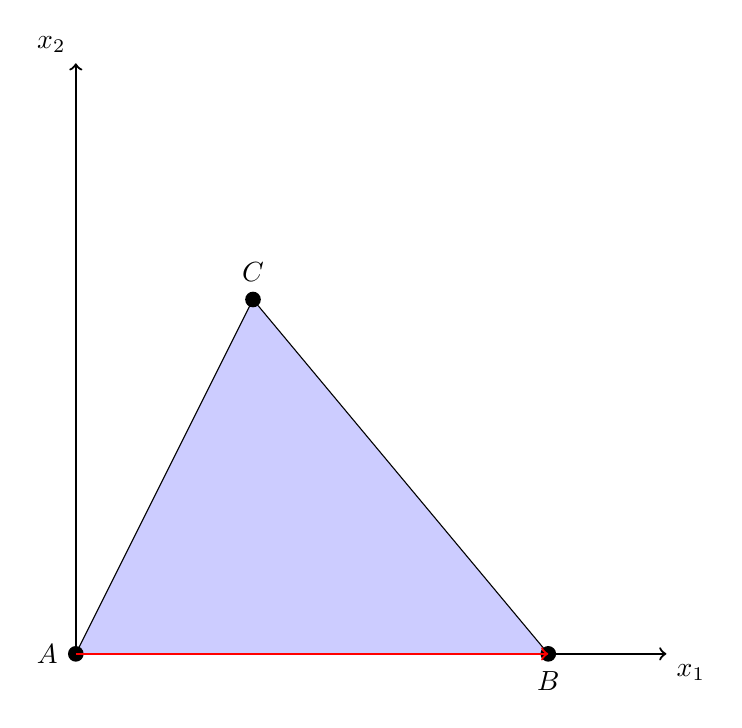
\begin{tikzpicture}[scale=1.5]
        % Draw axes
        \draw[thick,->] (0,0) -- (5,0) node[anchor=north west] {$x_1$};
        \draw[thick,->] (0,0) -- (0,5) node[anchor=south east] {$x_2$};

        % Draw polytope
        \filldraw[fill=blue!20] (0,0) -- (4,0) -- (1.5,3) -- cycle;

        % Label vertices
        \node at (0,0) [circle,fill,inner sep=2pt,label=left:{$A$}] {};
        \node at (4,0) [circle,fill,inner sep=2pt,label=below:{$B$}] {};
        \node at (1.5,3) [circle,fill,inner sep=2pt,label=above:{$C$}] {};

        % Draw movement of simplex algorithm
        \draw[red,thick,->] (0,0) -- (4,0);
    \end{tikzpicture}
\end{center}

In the above figure, the shaded region represents
the feasible region of a linear programming problem.
The simplex algorithm starts at vertex \(A\) and moves to
vertex \(B\) because \(B\) offers a better objective value.
The algorithm would continue navigating the vertices until
the optimal solution is found.
\begin{itemize}
    \item The simplex algorithm only evaluates the objective
          function at the vertices of the feasible region.
    \item At each step, the algorithm selects an adjacent
          vertex with a better objective value and moves to it.
    \item The algorithm terminates when it reaches a vertex where
          all adjacent vertices have worse objective values, indicating an
          optimal solution.
\end{itemize}
\subsubsection{The complexity}
%Worst case vs. average case
With $m<50$ and $m+n<200$, where $m$ and $n$ are the number of constraints and variables in the \gls{lp}
problem respectively, Dantzig observed that the number of iterations are usually less than $3m/2$
and only rarely going to $3m$. However, there is no proof that for every
problem the simplex algorithm for
 linear programming has a number of iterations or pivots that 
is majorized by a polynomial function.
In fact, Klee and Minty (1972) \parencite{klee1972good} constructed a worst-case example where
 $2^m -1$ iterations may be required, making the simplex'
worst-case time complexity exponential, which we denote by \( O(2^m) \).
It can be however argued that this is only one worst-case example. Indeed, the number 
of iterations usually encountred in practice or even in formal experimental studies of is much lower.
For packing linear programs, the worst-case time complexity of the Simplex algorithm
remains exponential, even though there exists polynomial time implementations for it.
\parencite{stille2010solution}.

\subsection{The interior point method}

\subsection{Revised Simplex Algorithm}
While the standard or tableau simplex algorithm maintains and updates the entire tableau in its 
dense form at each iteration, meaning when we perform the pivotting we have to update the entire matrix
using row operations, the revised simplex 
method uses the same recursion relations to transform only the inverse of the basis for each iteration, thus 
reducing the amount of writing at each step and overall memory usage.
This is explained in the following mathematical proof.
\subsubsection*{Mathematical proof}
Given a linear programming problem in standard form:
\begin{align*}
\text{maximize} \quad & c^T x \\
\text{subject to} \quad & Ax = b \\
& x \geq 0
\end{align*}
where \( A \) is an \( m \times n \) matrix, 
\( b \) is an \( m \times 1 \) vector, and 
\( c \) is an \( n \times 1 \) vector.


Partition \( x \) into basic (\( x_B \)) and non-basic (\( x_N \)) variables. 
Similarly, partition \( A \) into \( B \) (columns corresponding to \( x_B \)) 
and \( N \) (columns corresponding to \( x_N \)).

The constraints can be written as:
\begin{align*}
Bx_B + Nx_N &= b \\
x_B &\geq 0 \\
x_N &\geq 0
\end{align*}

From \( Bx_B + Nx_N = b \), when \( x_N = 0 \):
\[ x_B = B^{-1}b \]
This is the basic feasible solution if all entries of \( x_B \) are non-negative.

Compute the reduced costs:
\[ \bar{c}_N^T = c_N^T - c_B^T B^{-1} N \]
If all entries of \( \bar{c}_N^T \) are non-negative, 
then the current basic feasible solution is optimal.

If some entries of \( \bar{c}_N^T \) are negative, 
choose \( j \) such that \( \bar{c}_j < 0 \). Compute:
\[ d = B^{-1} A_j \]
If all entries of \( d \) are non-positive, the problem is unbounded.

Otherwise, compute the step length:
\[ \theta = \min \left\{ \frac{x_B[i]}{d[i]} : d[i] > 0 \right\} \]
Update the solution:
\[ x_B = x_B - \theta d \]
\[ x_j = \theta \]
and adjust the sets of basic and non-basic variables.

Repeat the optimality test, and if necessary, the pivot operation, 
until an optimal solution is found or the problem is determined to be unbounded. 

This proof elucidates that at every stage of the simplex method, we only have to
 track the following variables:
\begin{itemize}
    \item the indices of basic and non-basic variables
    \item $B^{-1}$ the inverse of the basis matrix. This is used to solve two types of linear equations
    during an iteration, see step 1 and 3 in \ref{algo:revised}.
    \item the current values of the basic variables, or the current basic feasible solution $x_B = B^{-1}b$
\end{itemize}
In practical terms, we only update the basis matrix every iteration, and we will be able to use it to
perform all the steps needed to update our problem data and go on to the next
iteration.
The algorithm is elaborated in \ref{algo:revised}. As we can see, step 1 and 3 represent the solving of
two types of systems , \gls{ftran} and \gls{btran}. This can be done using a multiplication with
the basis matrix inverse'. 

However, having to recompute the inverse of a matrix is costly.

For a square matrix of size \(n \times n\), the time complexity of LU decomposition 
\parencite{golub2013matrix}, 
which is one of the 
most prominent methods to invert a matrix is $O(n^3) $.

This is why it is desirable to employ another tool to efficiently
update the inverse of the basis matrix $B^{-1}$
without having to recompute it from scratch,
making it computationally more efficient for large-scale problems. Such tools are called update methods,
and we will later describe the \gls{pfi}, the modified \gls{pfi} and Forrest-Tomlin update method. 

Finally, in our implementation we also use the \gls{ccr} format to store matrices, 
see \ref{subsubsection:sparse-matrix} of the,
which greatly benefits the performance of the implementation.

\begin{algorithm}
    \caption{Revised Simplex Algorithm}
    \begin{enumerate}
        \item \textbf{Input:} A feasible basic solution, \( B \), \( c \), \( A \), and \( b \)
        \item \textbf{Output:} Optimal solution or a certificate of unboundedness
        \item Initialize \( B^{-1} \), the inverse of the basis matrix \( B \)
        \item \textbf{While True:}
              \begin{itemize}
                  \setlength{\itemindent}{3em}
                  \item[\textit{Step 1:}] Solve the system \( yB = c_B \) (BTRAN)
                  \item[\textit{Step 2:}] Choose an entering column. This may be any column a of
                      $A_N$ such that $ya$ is less than the corresponding component
                      of $c_N$. If there is no such column, then the current solution is optimal.
                      In other words: Choose first \( j \) such that \( c_j -yA_j > 0 \)
                      then $a=A_j$ is the enterig column.
                  \item[\textit{Step 3:}] Solve the system $Bd = a$ (FTRAN)
                  \item[\textit{Step 4:}] Let $x_B^{\ast} = B^{-1}b$ the current basic variables' values.
                      Find the largest $t$ such that \( x_B^{\ast} - td \geq 0\)
                      if there is no such $t$, then the problem is unbounded; otherwise, at least
                      one component of  \( x_B^{\ast} - td \) equals zero and the corresponding variable is leaving the basis.
                  \item[\textit{Step 5:}] Set the value of the entering variable at
                      $t$ and replace the values $x_B^{\ast}$ of the basic variables by \( x_B^{\ast} - td \).
                      Replace the leaving column of B by the entering column, and in the basis heading,
                      replace the leaving variable by the entering variable.
              \end{itemize}

        \item \textbf{Return} Optimal solution \( B^{-1}b \)
    \end{enumerate}
\end{algorithm}\label{algo:revised}

\subsubsection*{The product form inverse update method}
We will discuss the PFI, introduced by George Dantzig \parencite{dantzig1954product}.
The revised simplex method 
\subsection{Cardinality Estimation}\label{subsection:cardinality-estimate}
In the pipeline of query execution, cardinality estimation serves
as a cornerstone for the query optimization process.
Cardinality, defined as the number of tuples in the output,
plays a pivotal role in the selection of an optimal query plan.
Modern \gls{dbms} often rely on
cost-based query optimizers to make this selection.
For example, the SQL Server Query Optimizer
\parencite{microsoft2023cardinality} employs a
cost-based approach, aiming to minimize the estimated
processing cost of executing a query.

Enhanced cardinality estimation
can lead to more accurate cost models, which in turn results
in more efficient query execution plans.
Consequently, accurate and reliable cardinality estimates are
crucial in achieving faster query execution times.
The objective is to develop a \gls{lp}
solver designed specifically for cardinality estimation.
This solver aims to maximize a cost function that represents
the upper bound of the output size, optimizing for both
time and memory complexity.

To set the stage for our implementation,
we focus on the problem of upper-bounding the
cardinality of a join query $Q$.

\subsubsection{Scenario}
To elucidate the core concepts,
suppose we have two relation $R$ and $S$ with attributes 
\[
    Q(a, b, c) = R(a, b) \Join S(b, c)
\]
where we denote the sizes of the relations as
$|R|$ and $|S|$ respectively.
It is easy to see that the largest possible output is $|R| \cdot |S|$, which occurs when the join
behaves like a cartesian product, i.e. have a selectivity equals to 1. So, this is the worst-case
upper bound.
\subsubsection{AGM bound}
The AGM bound \parencite{atserias2013size} proves
using entropy that \[ \min_w \left( \sum_{i=1}^{k} w_i \log |R_i| \right) \]
is a tight upper bound for join size, given query graph (how the
relations are connected, if there are any shared attributes)
and relation sizes.
The dual \gls{lp} problem of the given minimzation problem, is
\[ \max \sum_{i} v_i \]
subject to:
\[ A^T \mathbf{v} \leq \log |R| \]
The dual theorem \ref{duality} states that the both problems have the same 
optimal values. 

This is how our \gls{lp} datasets are generated.

We start with the inequality \ref{eq:initial_inequality}. Applying the natural logarithm to both sides yields \ref{eq:log_inequality}. We then rename the variables, simplifying the inequality to \ref{eq:renamed_inequality}.
Normalizing by dividing both sides by \(r'\), we obtain \ref{eq:normalized_inequality}. This leads us to the objective function for our packing LP problem.
\begin{align}
    |a| \cdot |b|                            & \leq |R| \label{eq:initial_inequality}                                                   \\
    \ln|a| + \ln|b|                          & \leq \ln|R| \label{eq:log_inequality}                                                    \\
    a' + b'                                  & \leq r' \label{eq:renamed_inequality}                                                    \\
    \frac{1}{r'} a' + \frac{1}{r'} b'        & \leq 1 \label{eq:normalized_inequality}                                                  \\
    \text{maximize } a' + b' + c' + d' \quad & \text{s.t.} \quad \frac{1}{r'} a' + \frac{1}{r'} b' \leq 1 \label{eq:objective_function}
\end{align}

And in this simple abstracted way we get a sample packing LP from our dataset.
\subsubsection{Variables}
\subsubsection{Objective}
\subsubsection{Constraints}

\section{Previous Work}
Here we will discuss alternative approaches that are superseded by my work.
\subsection{Comparative studies of different update methods}
We will focus on one study \parencite{huangfu2015novel}.
\subsection{Other techniques}
The primal simplex method starts from a trial point that is primal feasible and iterates until dual feasibility.
The dual simplex method starts from a trial point that is dual feasible and iterates until primal feasibility.
ALGLIB implements a three-phase dual simplex method with additional degeneracy-breaking perturbation:
\begin{itemize}
    \item Forrest-Tomlin updates for faster LU refactorizations
    \item A bound flipping ratio test (also known as long dual step) for longer steps
    \item Dual steepest edge pricing for better selection of the leaving variable
    \item Shifting (dynamic perturbations applied to cost vector) for better stability
\end{itemize}
